\Opensolutionfile{solutions}[ex]
\section*{Exercises}

\begin{enumialphparenastyle}

\begin{ex}
Graphically, find the point $\tup{x,y}$ which
lies on both of the lines $x+3y=1$ and $4x-y=3$. That is, graph each line
and see where they intersect.

\begin{sol}
$\begin{array}{c}
x+3y=1 \\
4x-y=3
\end{array}$, Solution is: $\mat{x=\frac{10}{13},y=\frac{1}{13}}$.
\end{sol}
\end{ex}


\begin{ex}
Graphically, find the point of intersection of the two lines $
3x+y=3$ and $x+2y=1$. That is, graph each line
and see where they intersect. 

\begin{sol}
$\begin{array}{c}
3x+y=3 \\
x+2y=1
\end{array}
$, Solution is: $\mat{x=1,y=0} $
\end{sol}
\end{ex}

\begin{ex} You have a system of $k$ equations in two variables, $k\geq 2$.
Explain the geometric significance of

\begin{enumerate}
\item No solution.

\item A unique solution.

\item An infinite number of solutions.
\end{enumerate}

%\begin{sol}
%\end{sol}
\end{ex}

\begin{ex}
  Draw a picture of three planes such that no two of the planes are
  parallel, but the three points have no common intersection.

  \begin{sol}~\par\vspace{-2ex}\quad
    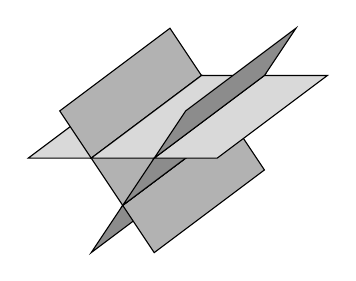
\begin{tikzpicture}[xscale=0.2,yscale=0.15]
      \draw[fill=gray!30] (-6,0) -- ++(7,7) -- ++(4,0) -- ++(-7,-7) -- cycle;
      \draw[fill=gray!90] (-2,-8) -- ++(7,7) -- ++(2,4) -- ++(-7,-7) -- cycle;
      \draw[fill=gray!60] (2,-8) -- ++(7,7) -- ++(-2,4) -- ++(-7,-7) -- cycle;
      \draw[fill=gray!60] (0,-4) -- ++(7,7) -- ++(-2,4) -- ++(-7,-7) -- cycle;
      \draw[fill=gray!60] (-2,0) -- ++(7,7) -- ++(-2,4) -- ++(-7,-7) -- cycle;
      \draw[fill=gray!30] (-2,0) -- ++(7,7) -- ++(4,0) -- ++(-7,-7) -- cycle;
      \draw[fill=gray!90] (0,-4) -- ++(7,7) -- ++(2,4) -- ++(-7,-7) -- cycle;
      \draw[fill=gray!30] (2,0) -- ++(7,7) -- ++(4,0) -- ++(-7,-7) -- cycle;
      \draw[fill=gray!90] (2,0) -- ++(7,7) -- ++(2,4) -- ++(-7,-7) -- cycle;
    \end{tikzpicture}
  \end{sol}
\end{ex}

\end{enumialphparenastyle}
